\chapter{The Standard Model of particle physics}

The \ac{SM} of particle physics is our current best theoretical framework underpinning our understanding of the subatomic world, providing a description of fundamental elementary particles and their interactions via the electromagnetic force, weak nuclear force and the strong nuclear force. The fourth fundamental force of nature, Gravity, is absent from the SM, highlighting one of its key limitations. However, in high-energy physics experiments, where the interactions of subatomic particles are being studied, the omission of gravity is considered a safe simplification. Extremely powerful predictions have emerged from this theoretical framework, with its greatest success being the discovery of the Higgs boson by the ATLAS and CMS Collaborations in 2012, completing the observational confirmation of all hypothesized SM particles. Despite its success, the Standard Model has its limitations. Along with the absence of gravity, it leaves several fundamental questions unanswered, such as the nature of neutrino oscillations, the existence of dark matter, the hierarchy problem, and the matter-antimatter asymmetry in the universe, which cannot be fully explained by the predicted amount of CP violation, driving the field to look for explanations beyond the SM. In the pursue of \ac{BSM} physics, a deep understanding of the SM theory is crucial. This is the goal of this chapter aiming to establish the base foundation for this work, the SM, taking a trip down the fundamental blocks of the theory, including its particle content, interactions, and the Higgs mechanism.

\section{Particle content}

\begin{figure}
\centering
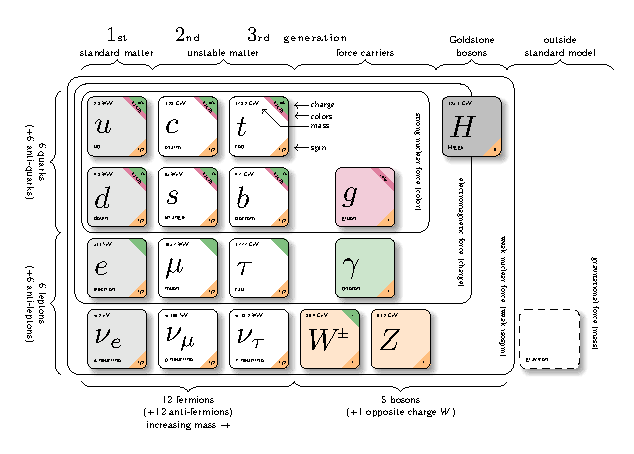
\includegraphics[width= 1\textwidth]{Figures/Introduction/Particles.pdf}
\end{figure}

\section{Fundamental forces}
\section{Higgs mechanism}
\section{The Higgs boson}

\cite{Rowling_1997}
\cite{Thor_2011}